\section{Wifi Security}

\subsection{Basic concepts of WiFi}
\paragraph{Terminology}
\begin{itemize}
    \item Station (STA) or client: terminal with access to wireless media.
    \item Access Point (AP): Station integrated to wireless media and distribution system.
    \item Basics service set (BSS): Group of stations using same radio frequency.
\end{itemize}

\paragraph{Channels:} 
\begin{itemize}
    \item WiFi standards provide radio frequency ranges, typically 2.4 or 5 GHz
    \item Each range is divided into several channels with 5MHz spacing
\end{itemize}

\begin{minipage}{\linewidth}
    \centering      
    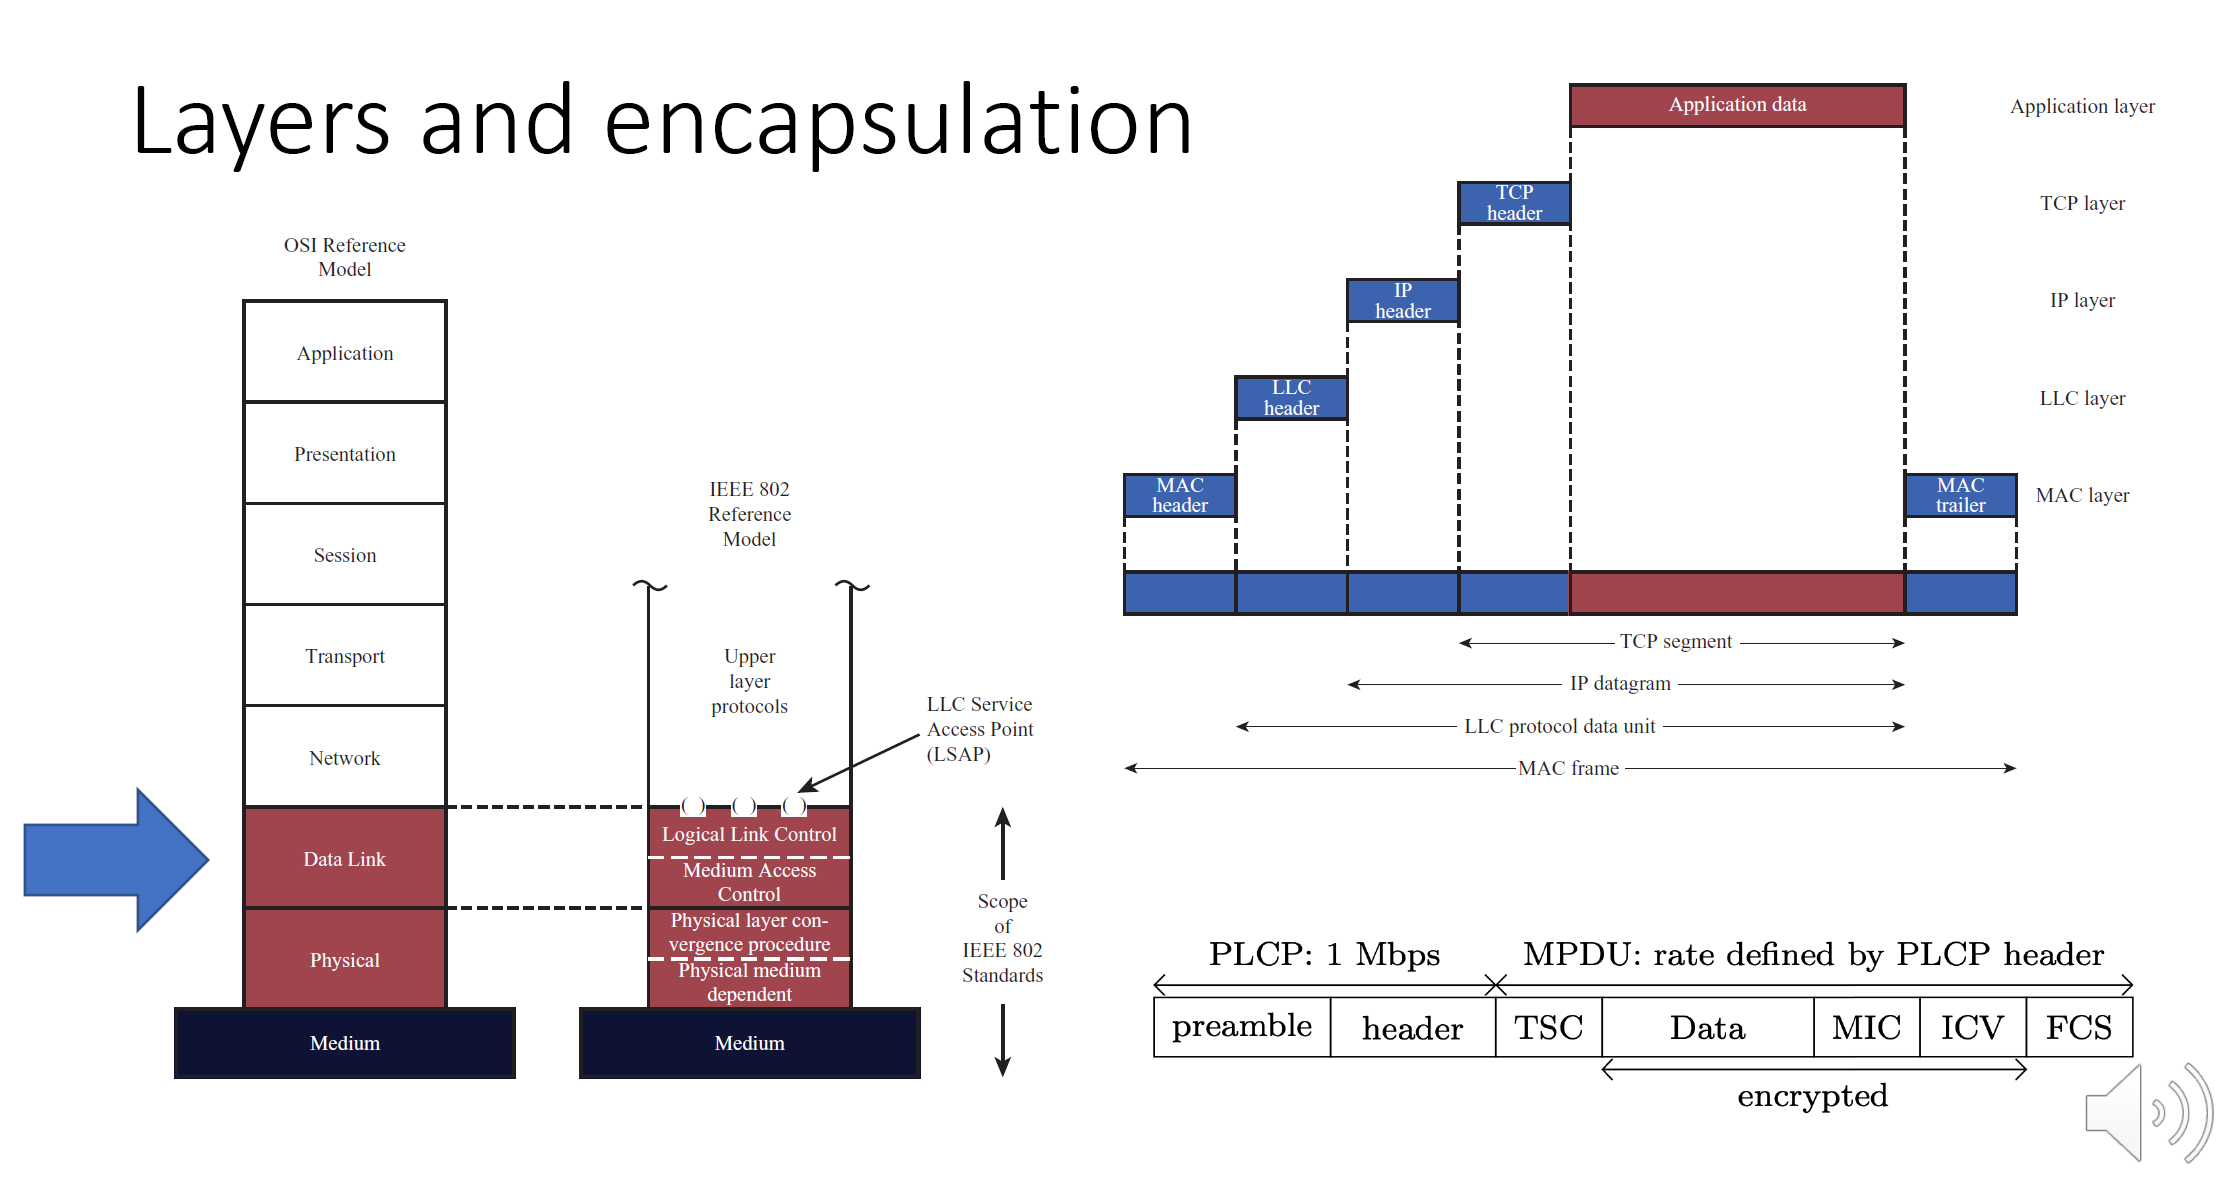
\includegraphics[width=\linewidth]{Figures/L9_layers.PNG}
\end{minipage}

\paragraph{Medium Access Control}
\begin{itemize}
    \item Multiple devices share the same communication medium.
    \item Goals: Reliable data delivery, Security
    \item Why handle these services at MAC layer? Can be more efficient than higher layer (e.g. tcp), can be safer than rely on applications or higher layer protocols.
\end{itemize}

\paragraph{CSMA/CA:} Carrier-Sense Multiple Access with collisiona avoidance, this entire mechanism is the Distributed Coordination Function (DCF)
\begin{enumerate}
    \item Carrier sense: prior to sending, check if medium is idle.
    \item Collision avoidance: If another node detected, wait for randomized "backoff period".
    \item Transmit entire frame, wait for ACK, if no ACK, wait for backoff period.
\end{enumerate}

\paragraph{Hidden node problem:} E.g. B can communicate with A and C and A cannot communicate with C.
Potential solution: After backoff transmit Request to send (RTS) to AP, wait for Clear to send (CTS) from AP

\paragraph{Frames:} allow 3-4 addresses (usually: sender, AP, destination). Frame types are Data, Control, Management (e.g. power)

\paragraph{Basic security goals:}
\begin{itemize}
    \item Communication security (confidentiality, integrity)
    \item Access contol (authentication)
    \item Communication fairness (equal throughput)
\end{itemize}

\subsection{Basic Manipulations}

\paragraph{Communication Fairness:} 
\begin{itemize}
    \item Previously mentioned DCF is proven to be fair, assuming all stations follow the rules.
    \item Unfair channel usage: Modify the driver to not backoff.
    \item if all stations use selfish backoff, then throughput will vary because of collisions, but only station with the strongest signal will be able to send
\end{itemize}

\paragraph{Simple Jamming:} How to turn your WiFi device into continuous jammer?
\begin{enumerate}
    \item Disable carrier sense
    \item Reset interframe space and disable backoff
    \item Don't wat for ACK
    \item Queue large number of frames for transmission
\end{enumerate}
Different ways to block WiFi frames: Trigger carrier sens of transmitter, or Mangle the frame at receiver (prevent receiving, need more power)

\paragraph{Selective Jamming:} Listen, Decode prefix of incoming frame, decide whether to jam. But one needs to be fast!

\paragraph{Man-in-the-middle position:}
\begin{itemize}
    \item Useful building block for many attacks
    \item Why not selective jamming? Success rate not 100\%
    \item Main idea: Clone AP on a different channel, forward frames from fake AP to real AP.
    \item How to make victims connect to fake AP? 
    \begin{itemize}
        \item Selectively jam beacons/probes (may not work)
        \item Continuously jam real AP -> clients switch (probably works)
    \end{itemize}
\end{itemize}

\subsection{WiFi Security Standards}

\subsubsection{WEP}
\begin{itemize}
    \item first WiFi security standard (1997)
    \item Goal: provide some level of communication protection (Confidentiality, Integrity, Access control)
    \item few years later WEP fully broken
    \item Checksum: Compute plaintext P = (M, c(M)), used for integrity protection (not a good idea!)
    \item Encryption: Encrypt using RC4 stream cipher, C = P xor RC4(IV, k)
    \item Send (IV, C)
\end{itemize}

\begin{minipage}{\linewidth}
    \centering      
    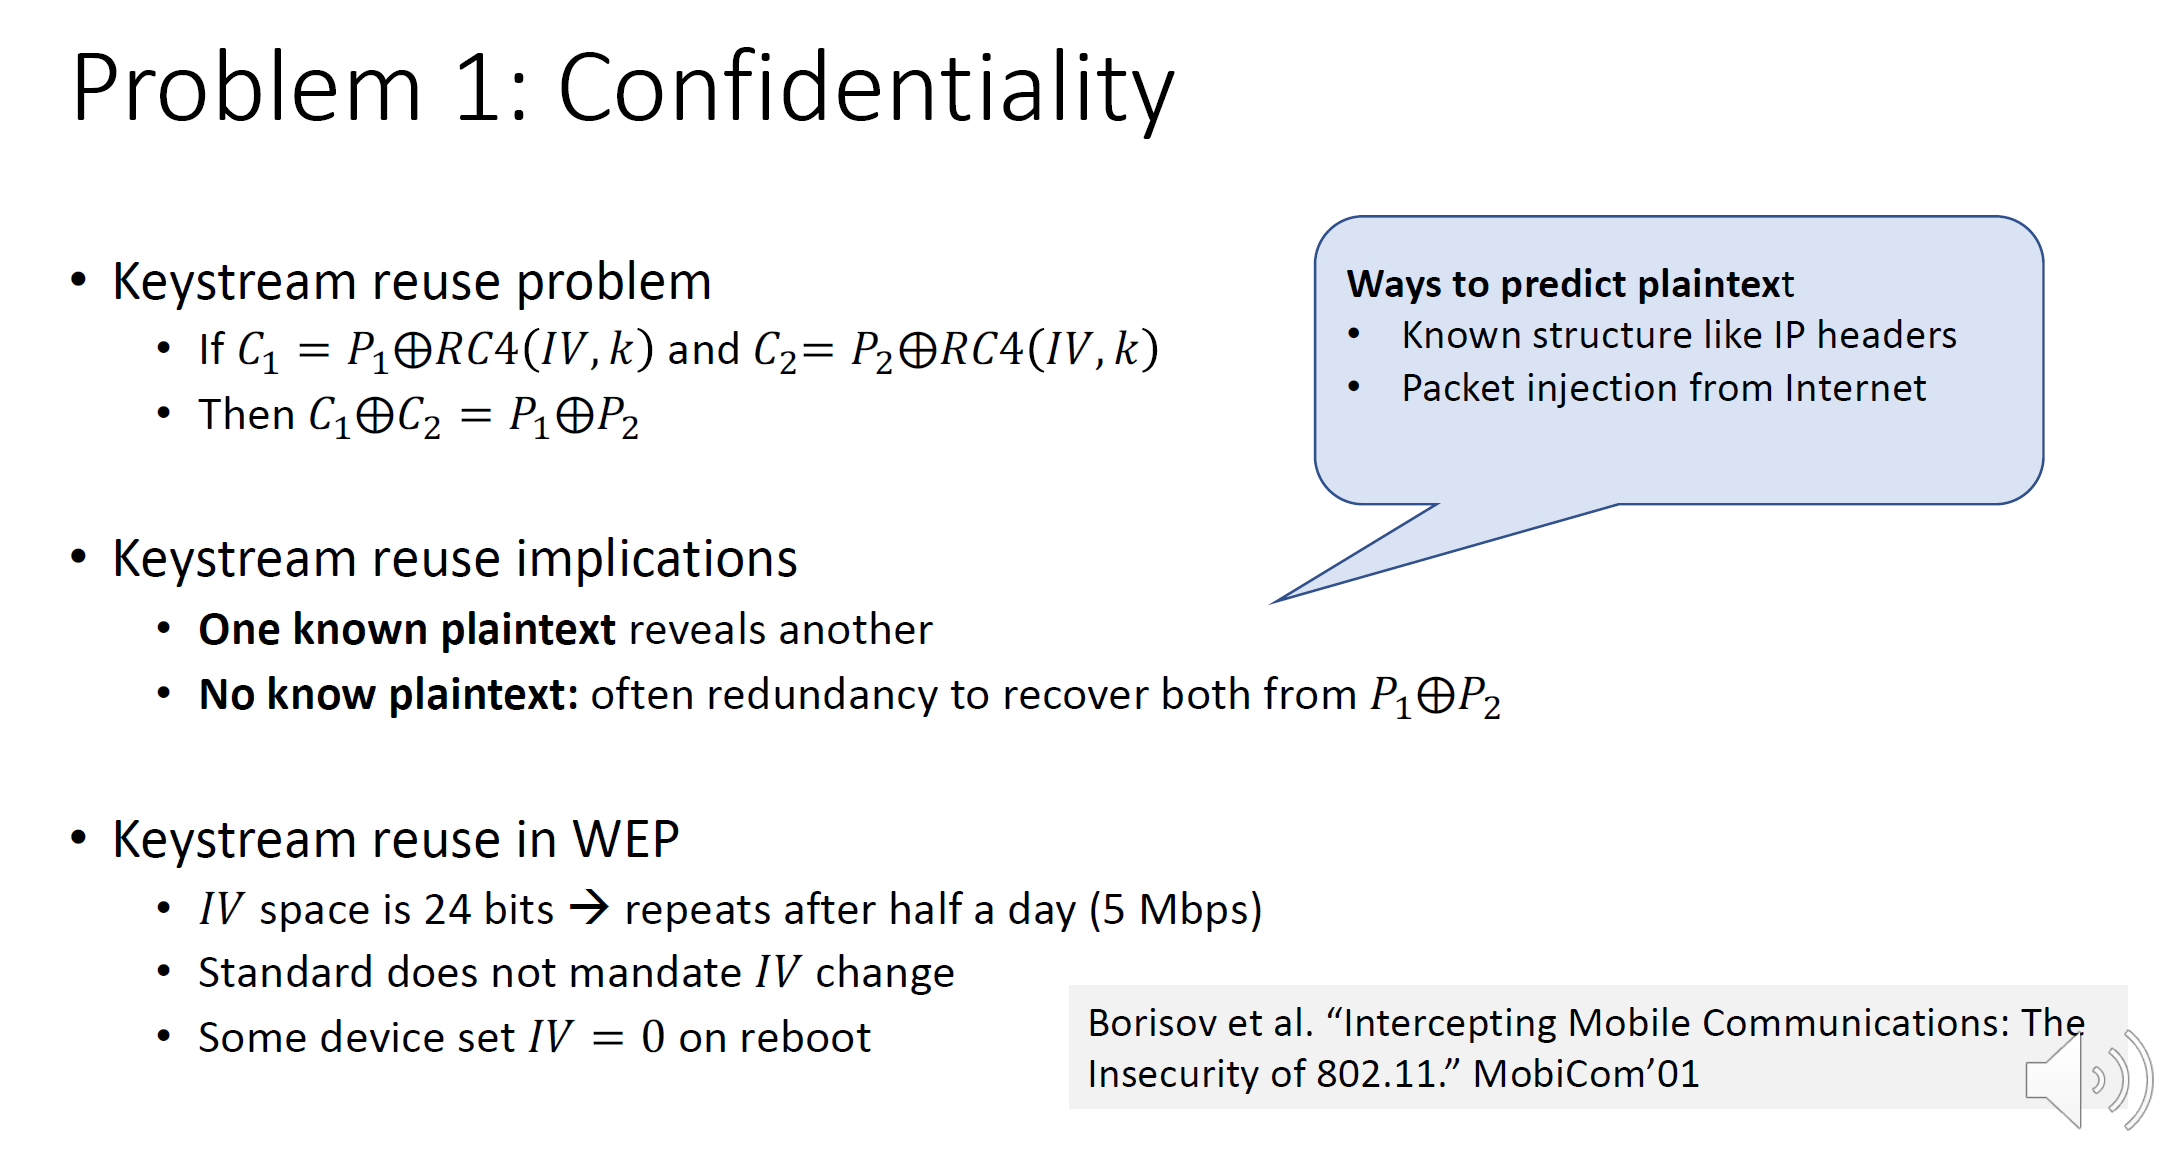
\includegraphics[width=\linewidth]{Figures/L9_wep_problem1.PNG}
\end{minipage}

\paragraph{Problem 2: Integrity}
The checksum used (CRC-32) is not a cryptographic MAC. Controlled message modifications are possible. 

\paragraph{Problem 3: Access Control}
\begin{enumerate}
    \item AP sends challenge in plaintext
    \item Station replies with WEP encryption of challenge (proof of key posession)
    \item AP completes network association
    \item [-] Simple attack: Monitor legitimate authetication -> learn plaintext/ciphertext pair.
    Derive Keystream (xor), compute valid response for new challenge.
\end{enumerate}

\subsubsection{WPA / TKIP}

\begin{itemize}
    \item The second WiFi security standard (2003) Wifi Protected Access (WPA)
    \item Main challenge: Design that works with legacy (WEP) devices, Firmware or driver update
    \item Goals: No keystream reuse, cryptographic MAC
    \item Constraints: Compatible with RC4/WEP hardware
    \item Enhancements: Augment encryption with per-packet key mixing. RC4 keystream filtering. New integrity protection mechanism (MICHAEL). Replay protection using counters (TSC)
\end{itemize}

\begin{minipage}{\linewidth}
    \centering      
    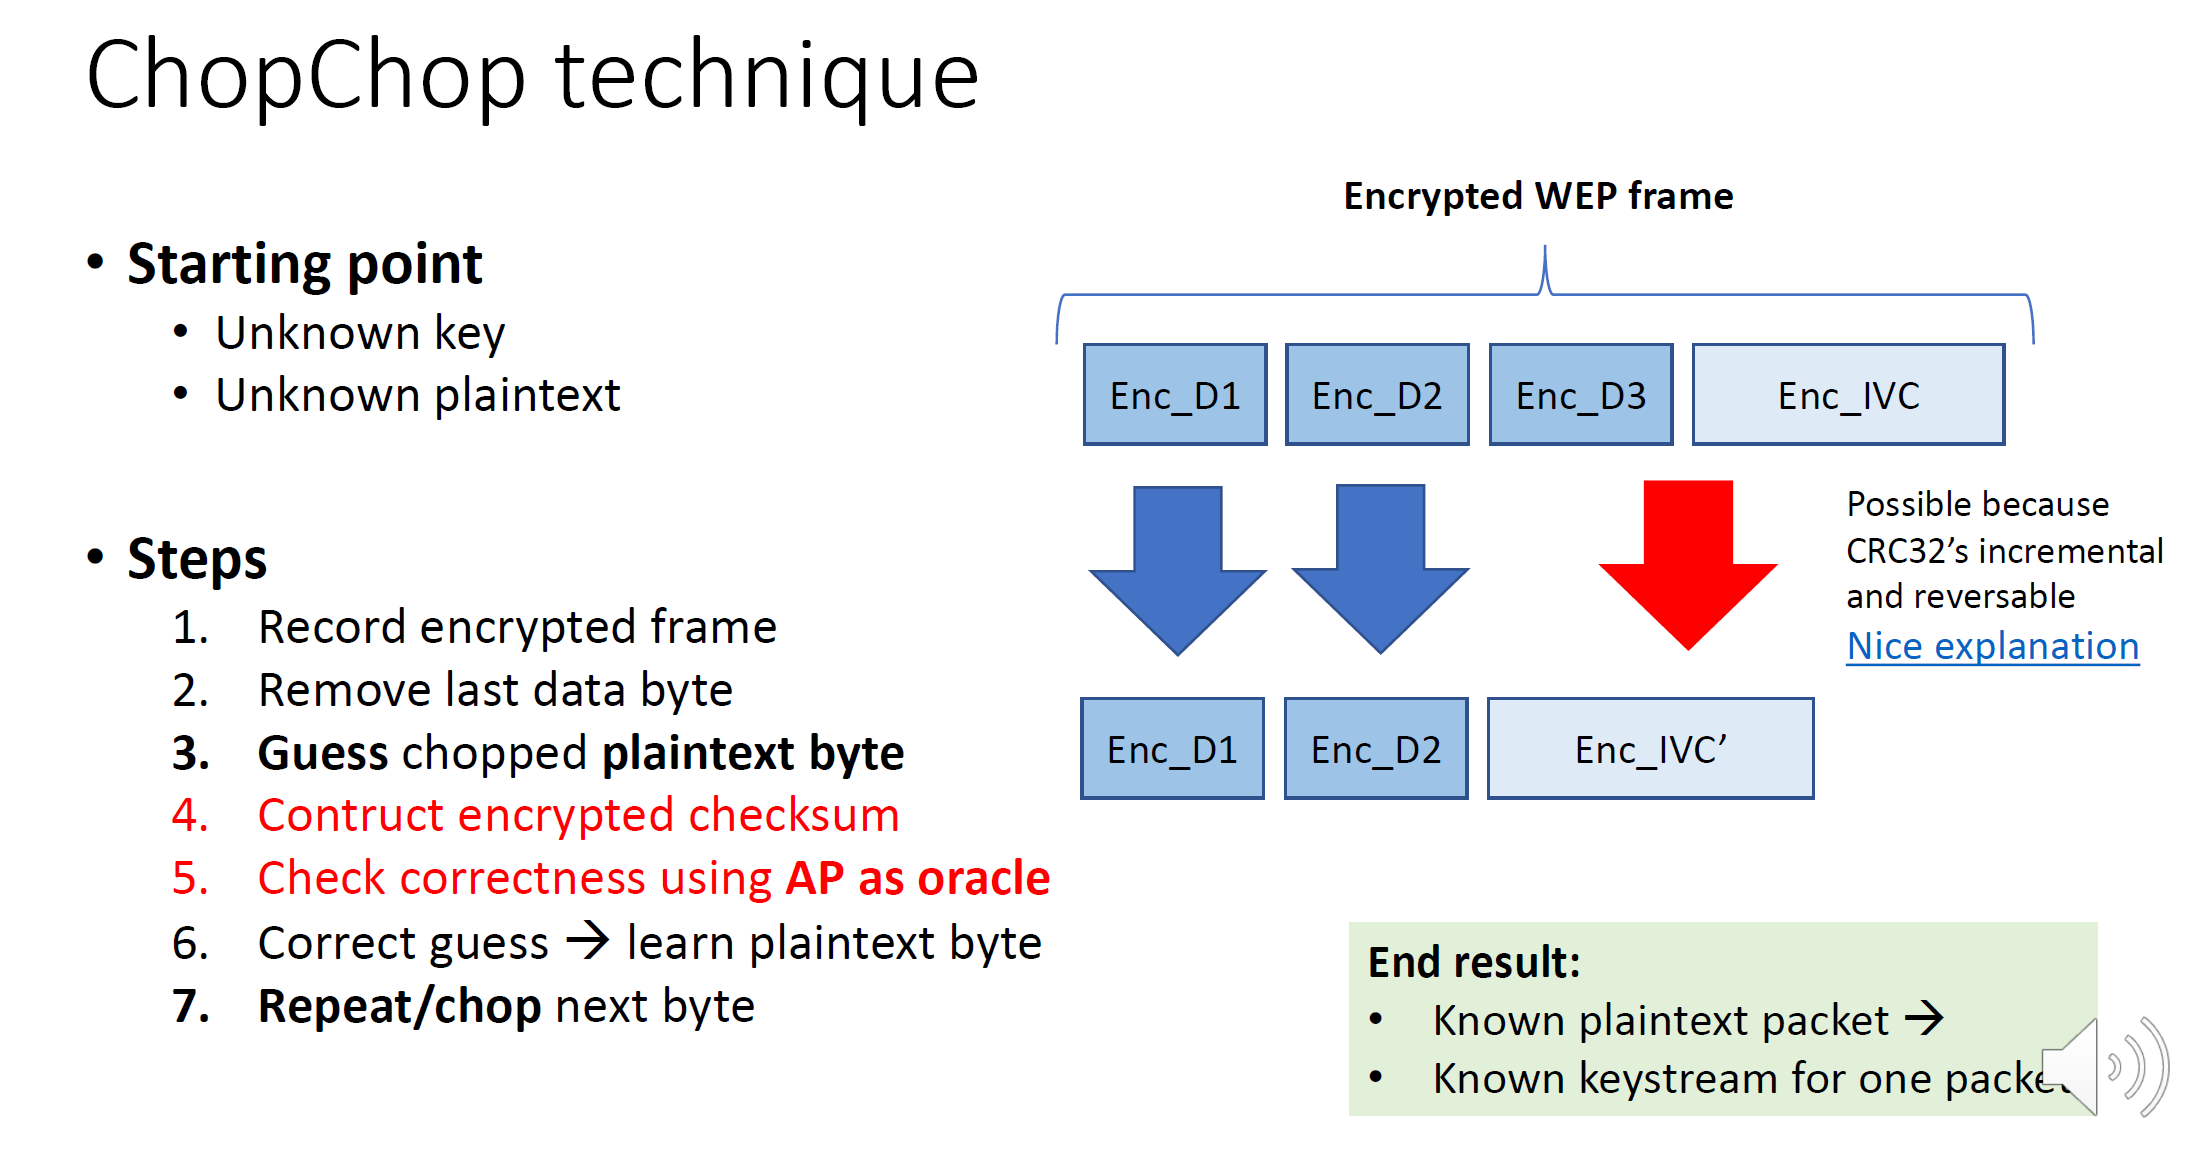
\includegraphics[width=\linewidth]{Figures/L9_chop_chop.PNG}
\end{minipage}

\begin{minipage}{\linewidth}
    \centering      
    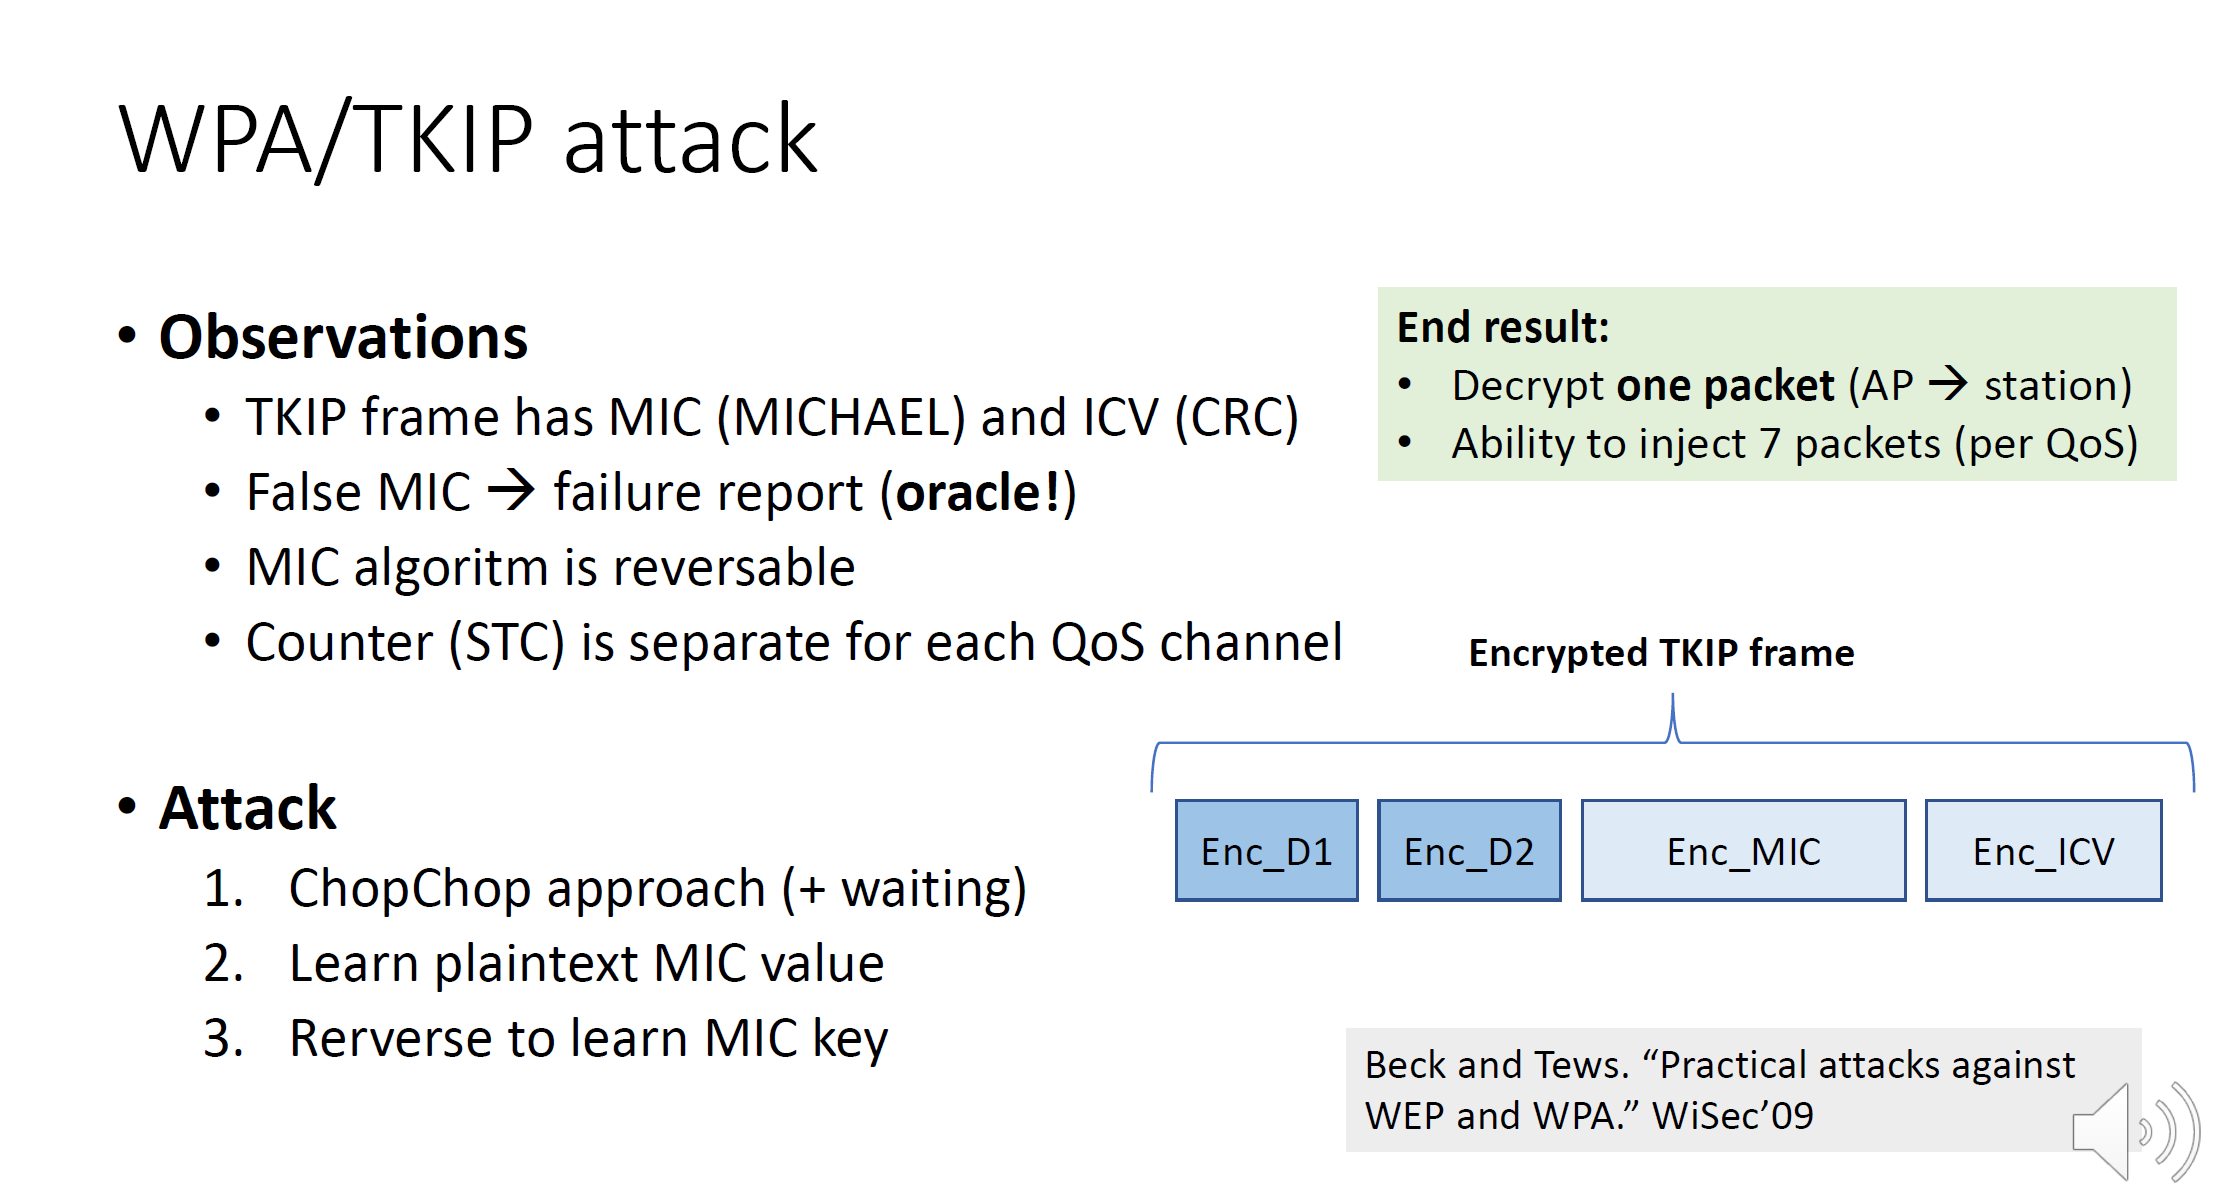
\includegraphics[width=\linewidth]{Figures/L9_wpa_attack.PNG}
\end{minipage}

\paragraph{Another Attack:} Statistical tests reveal biases in WPA/TKIP key stream.

\subsection{WPA2}
\begin{itemize}
    \item Introduced in 2004
    \item Better communication protection. Confidentiality using AES-128 in counter mode, Integrity usin CBC-MAC, Authenticate then encrypt
    \item WPA2 Handshake supports mutual authentication, session key agreement (PTK)
    \item Protocol proven secure in 2005
    \item Vulnerable to dictionary attacks: The handshake contains a MIC (Message Integrity Code) which makes it vulnerable to dictionary attack.
    Once the adversary has the MIC, he can try to compute it himself with guessed passwords and compare it with the captured MIC. That way, the adversary can bruteforce all possible passwords from a dictionary offline without having to interact with the AP.
\end{itemize}

\begin{minipage}{\linewidth}
    \centering      
    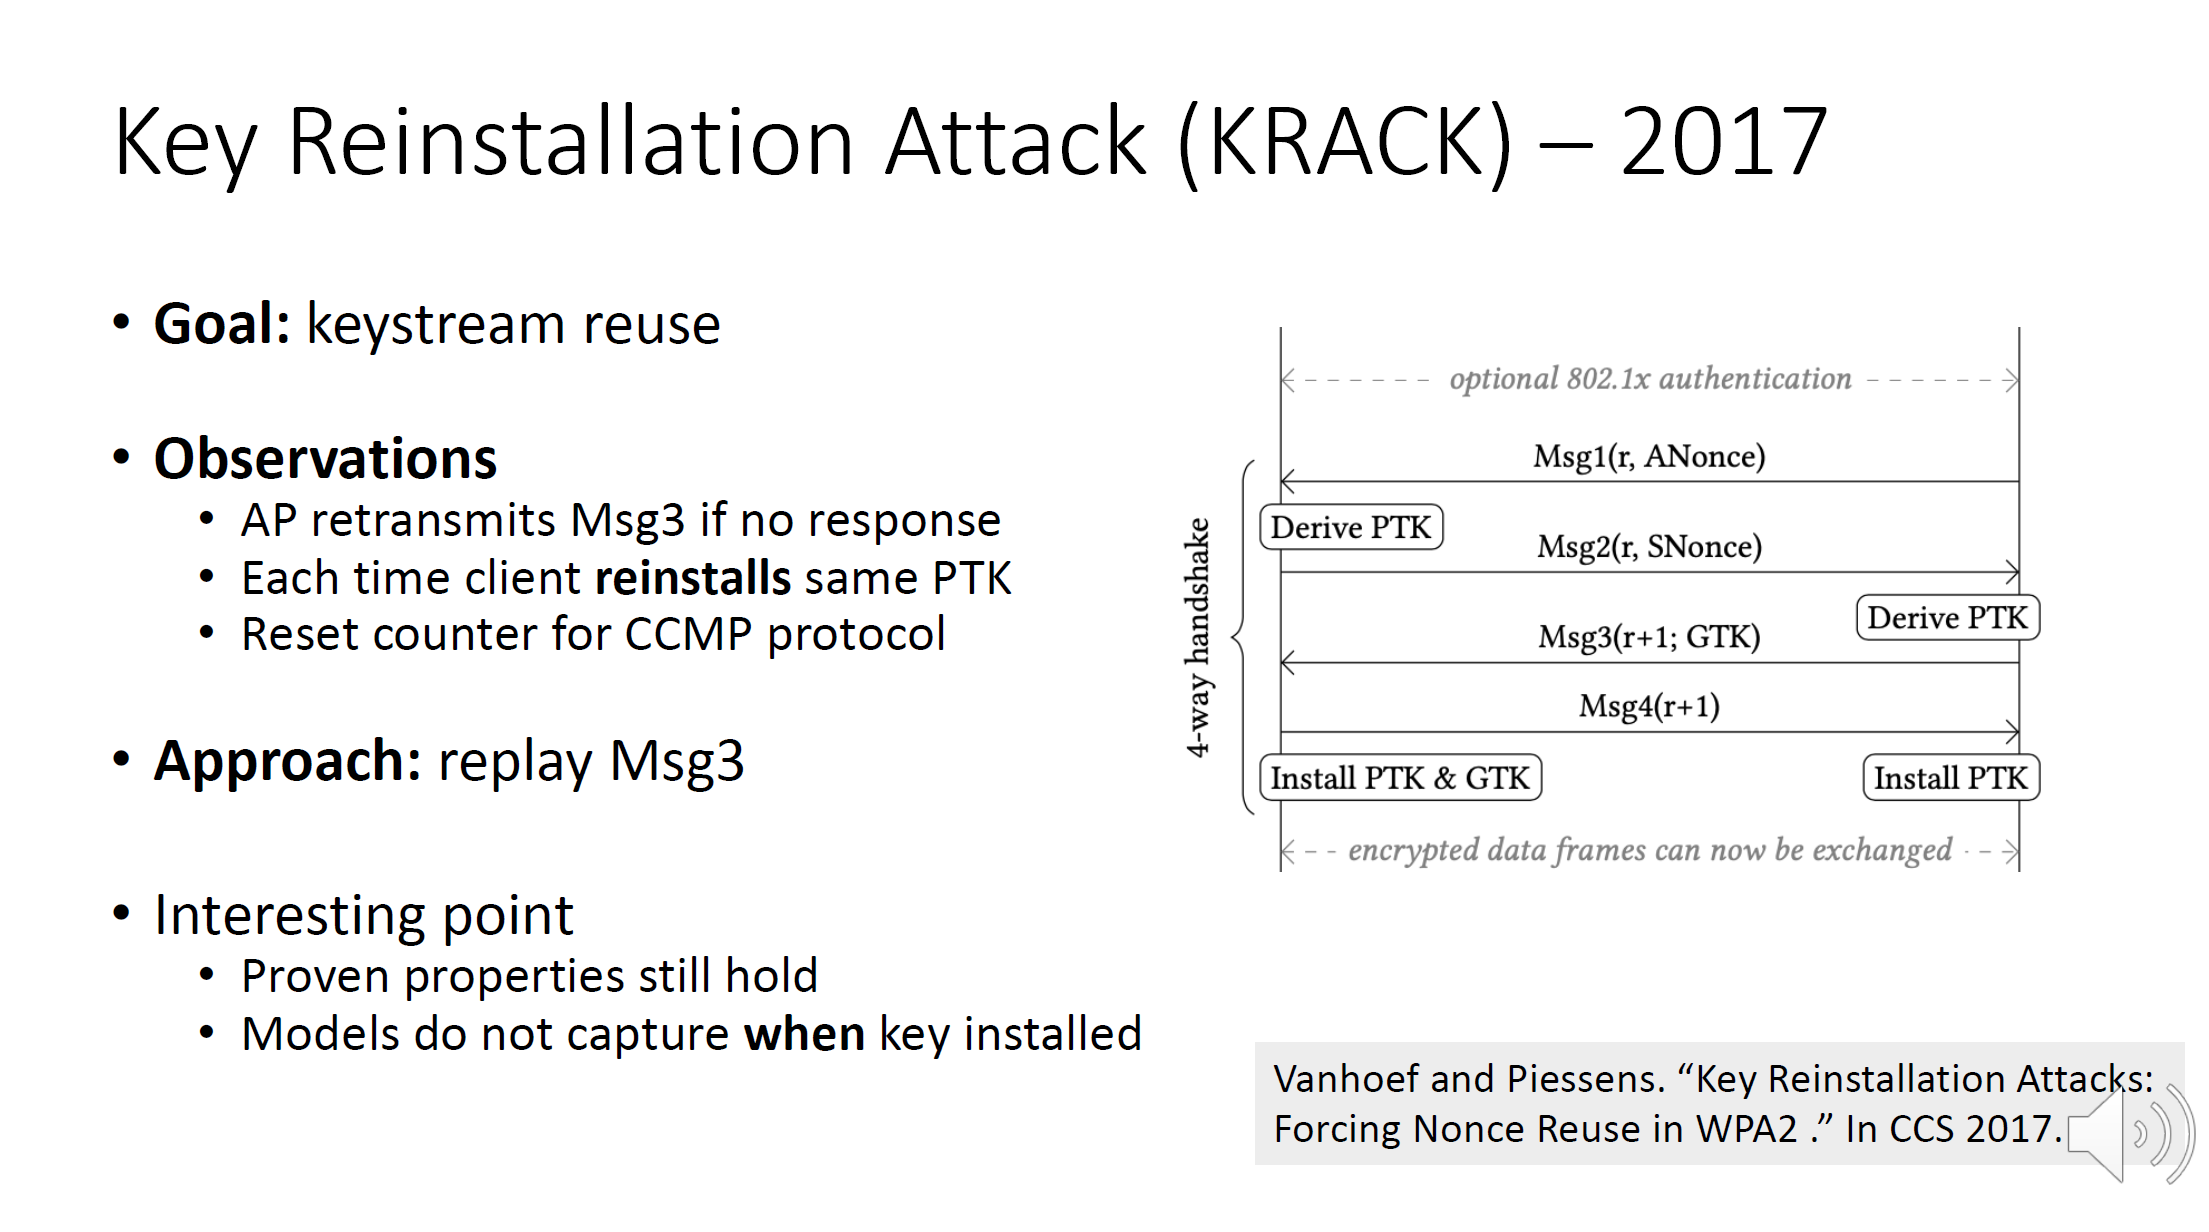
\includegraphics[width=\linewidth]{Figures/L9_krack.PNG}
\end{minipage}

\subsubsection{WPA3}
\begin{itemize}
    \item The latest WiFi security standard
    \item Updated crypto: confidentiality using AES-128, Integrity using SHA-384 HMAC
    \item New Handshake: Password-based authentication and key agreement
\end{itemize}

\begin{minipage}{\linewidth}
    \centering      
    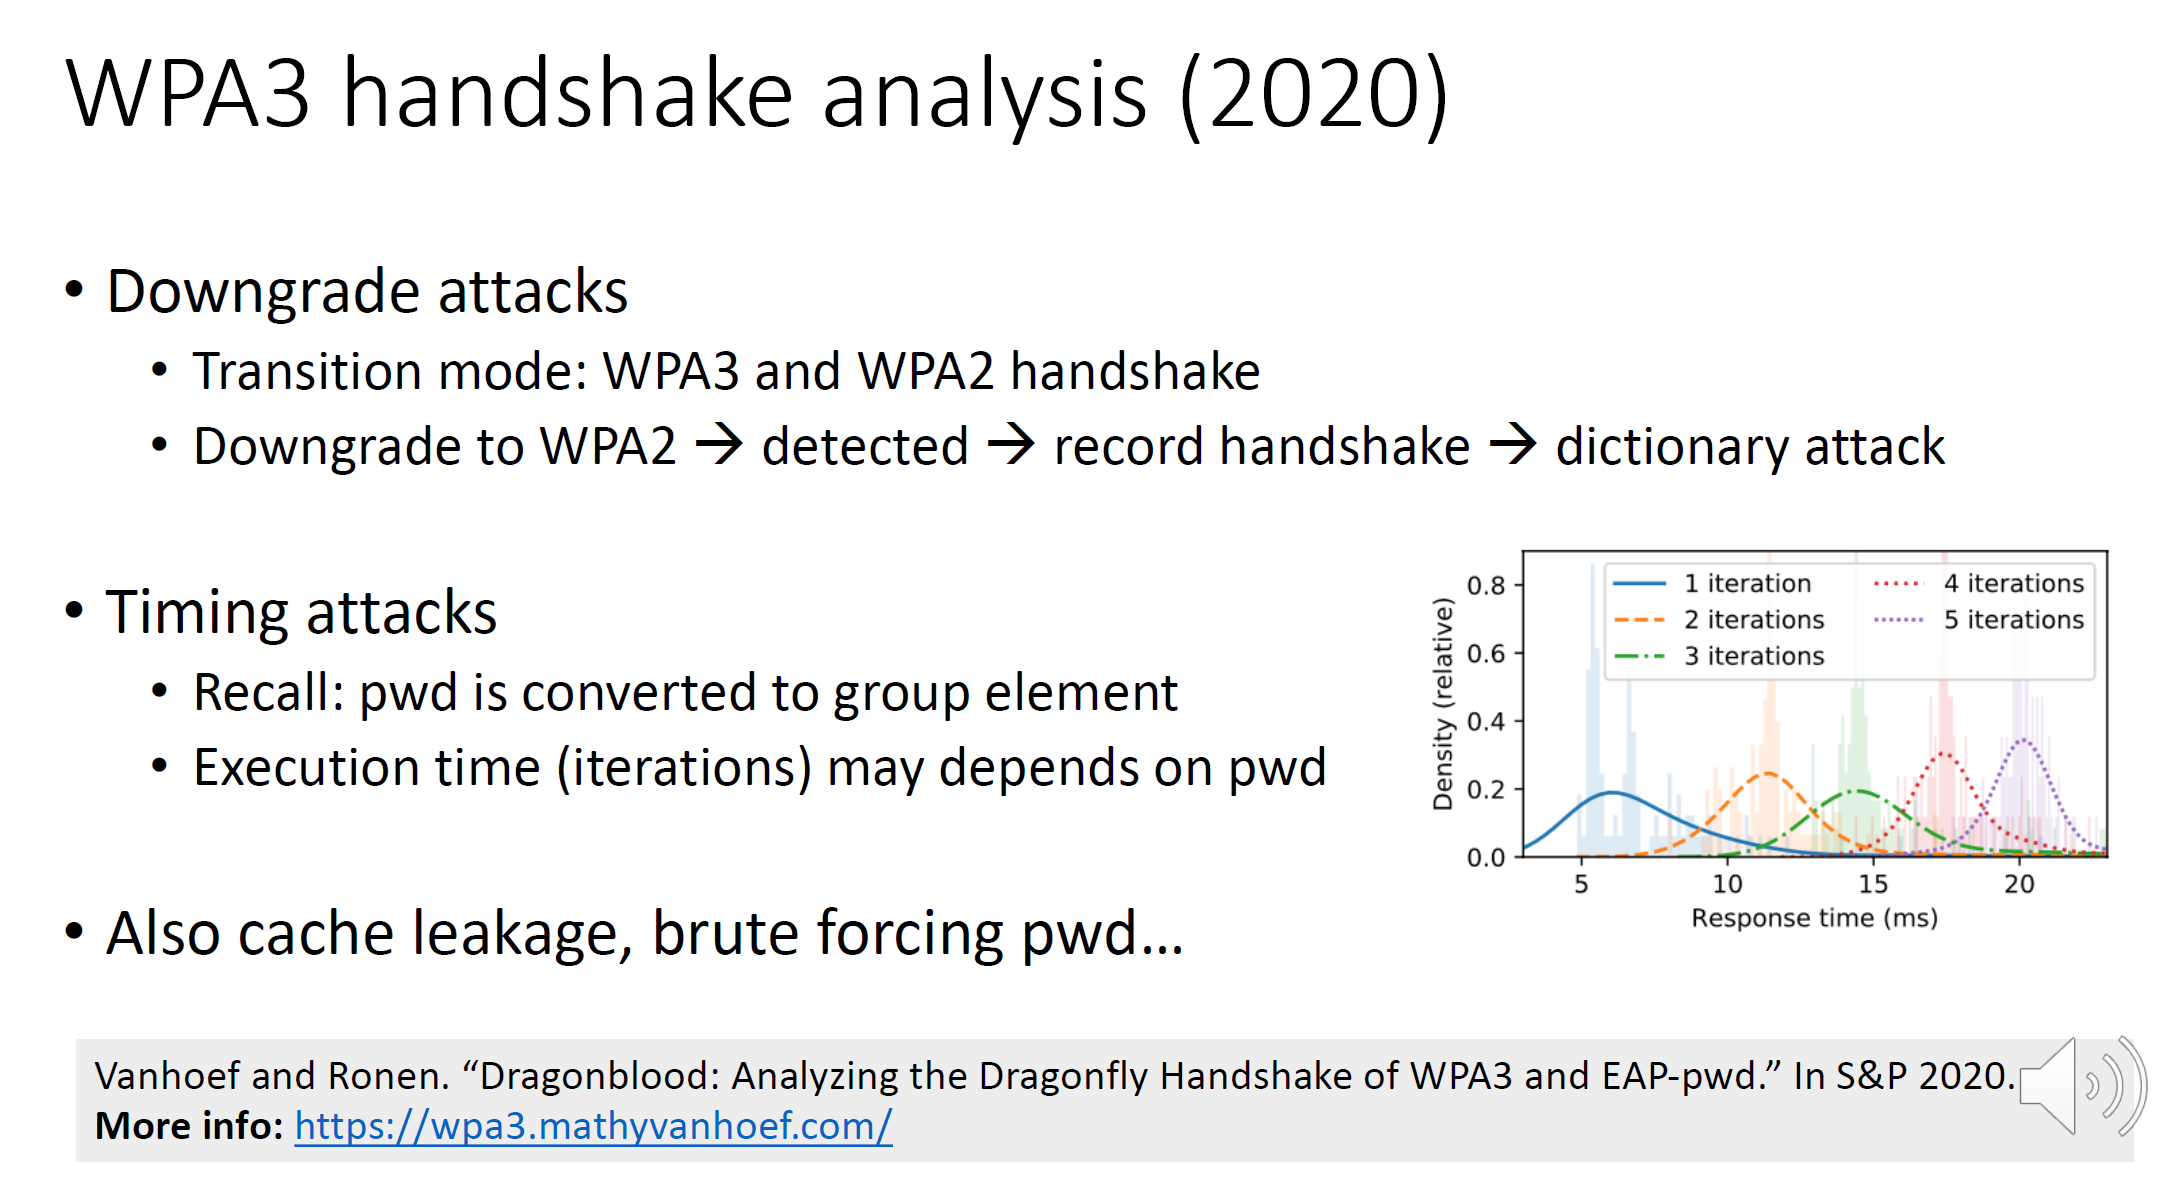
\includegraphics[width=\linewidth]{Figures/L9_wpa3_analysis.PNG}
\end{minipage}